\begin{pastexam}[label={px:ntu-110-dsaa-08}]{臺大資工所 110 學年度 第 VIII 題}
（單選；每格答對 5 分，答錯倒扣 2.5 分）

Given the following graph, try to find its minimum spanning tree.

\begin{center}
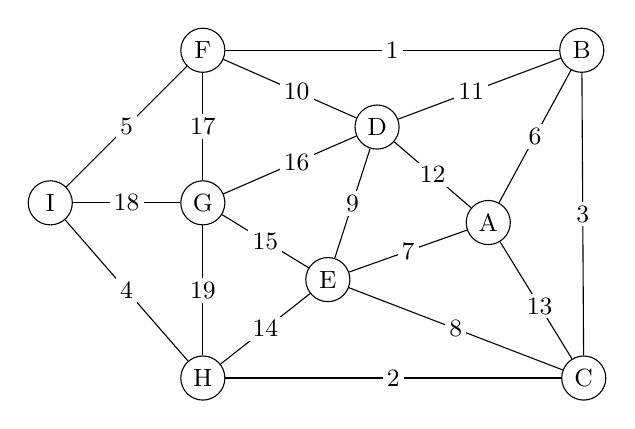
\begin{tikzpicture}[x=1.25cm,y=1.25cm,v/.style={circle,draw,inner sep=0pt,minimum size=5.6mm,font=\small},w/.style={fill=white,inner sep=1.5pt,font=\small}]
\node[v] (F) at (2.1,-0.5) {F};
\node[v] (B) at (5.95,-0.5) {B};
\node[v] (D) at (3.87,-1.28) {D};
\node[v] (I) at (0.55,-2.05) {I};
\node[v] (G) at (2.1,-2.05) {G};
\node[v] (A) at (5.0,-2.25) {A};
\node[v] (E) at (3.37,-2.83) {E};
\node[v] (H) at (2.1,-3.83) {H};
\node[v] (C) at (5.97,-3.83) {C};
\draw (F)--node[w]{1}(B);
\draw (F)--node[w,pos=0.55]{10}(D);
\draw (F)--node[w]{17}(G);
\draw (F)--node[w]{5}(I);
\draw (D)--node[w,pos=0.45]{11}(B);
\draw (D)--node[w,pos=0.45]{16}(G);
\draw (D)--node[w]{12}(A);
\draw (D)--node[w]{9}(E);
\draw (B)--node[w]{6}(A);
\draw (B)--node[w]{3}(C);
\draw (I)--node[w]{18}(G);
\draw (I)--node[w]{4}(H);
\draw (G)--node[w]{15}(E);
\draw (G)--node[w]{19}(H);
\draw (A)--node[w]{7}(E);
\draw (A)--node[w,pos=0.55]{13}(C);
\draw (E)--node[w]{14}(H);
\draw (E)--node[w]{8}(C);
\draw (H)--node[w]{2}(C);
\end{tikzpicture}
\end{center}
\begin{enumerate}[label=(\alph*)]
\item What is the sixth edge that Kruskal's algorithm includes (the numbering of the inclusion
order starts from 1, not 0)? \underline{\makebox[5em]{(14)}}

(A) 6 \qquad (B) 7 \qquad (C) 8 \qquad (D) 9
\item What is the sixth vertex that Prim's algorithm includes if starting from vertex A (the
numbering of the inclusion order starts from 1, \textbf{not} 0)? \underline{\makebox[5em]{(15)}}

(A) C \qquad (B) E \qquad (C) H \qquad (D) I
\end{enumerate}
\end{pastexam}

\begin{pastsoln}
答案：(14) 選 (B) 7；(15) 選 (D) I。

圖有 $9$ 個頂點、$19$ 條邊，權重 $1$--$19$ 各出現一次，全部不同，所以最小生成樹只有一棵（資結書
定理~24.4），兩個演算法找到的是同一棵樹，只是加入的順序不同。 (14) 的選項是權重，邊就用權重
稱呼。

\textbf{(14) Kruskal}（資結書第~24.2~節）：邊依權重由小到大看，兩端已經在同一個集合（加進來會
成環）就跳過，否則加入並合併兩個集合。
\begin{center}
\small
\begin{tabular}{cclll}
\toprule
權重 & 邊 & 結果 & 第幾條 & 加入後的集合（只列兩個點以上的） \\
\midrule
1 & F--B & 加入 & 1 & $\{B, F\}$ \\
2 & H--C & 加入 & 2 & $\{B, F\}$, $\{C, H\}$ \\
3 & B--C & 加入 & 3 & $\{B, C, F, H\}$ \\
4 & I--H & 加入 & 4 & $\{B, C, F, H, I\}$ \\
5 & F--I & 跳過（F、I 同集合） & & \\
6 & B--A & 加入 & 5 & $\{A, B, C, F, H, I\}$ \\
7 & A--E & 加入 & \textbf{6} & $\{A, B, C, E, F, H, I\}$ \\
8 & E--C & 跳過（E、C 同集合） & & \\
9 & D--E & 加入 & 7 & $\{A, B, C, D, E, F, H, I\}$ \\
10--14 & & 都跳過（兩端都已在同一集合） & & \\
15 & G--E & 加入 & 8 & 全部 $9$ 個點 \\
\bottomrule
\end{tabular}
\end{center}
第 $10$ 到 $14$ 的邊是 F--D、D--B、D--A、A--C、E--H，兩端都在那個 $8$ 個點的集合裡。 加到第 $8$
條邊（$= 9 - 1$）就停。 第六條加入的是權重 $7$ 的 A--E，選 (B)。 (A) 6 是第五條；(C) 8 的 E--C
會和 E--A--B--C 成環，被跳過；(D) 9 是第七條。

\textbf{(15) Prim}（資結書第~24.3~節）：從 A 開始，每一步加入「一端在樹裡、一端不在」的邊裡最輕
的那一條的另一端。 A 本身是第 $1$ 個。
\begin{center}
\small
\begin{tabular}{clll}
\toprule
第幾個 & 加入 & 經由的邊 & 當時其他跨越邊裡較輕的幾條 \\
\midrule
1 & A & （起點） & \\
2 & B & A--B 6 & A--E 7, A--D 12, A--C 13 \\
3 & F & B--F 1 & B--C 3, A--E 7, B--D 11 \\
4 & C & B--C 3 & F--I 5, A--E 7, F--D 10 \\
5 & H & C--H 2 & F--I 5, A--E 7, C--E 8 \\
6 & \textbf{I} & H--I 4 & F--I 5, A--E 7, C--E 8 \\
7 & E & A--E 7 & C--E 8, F--D 10, E--H 14 \\
8 & D & E--D 9 & F--D 10, E--G 15 \\
9 & G & E--G 15 & D--G 16, F--G 17 \\
\bottomrule
\end{tabular}
\end{center}
第六個加入的是 I，選 (D)。 (A) C 是第四個，(C) H 是第五個，(B) E 是第七個。 注意 I 是經由
H--I（權重 $4$）加入的，不是 F--I（權重 $5$）：第 $5$ 步加入 H 以後，H--I 比 F--I 輕。

兩個演算法得到的樹都是 $\{1, 2, 3, 4, 6, 7, 9, 15\}$ 這八條邊，總權重 $47$。
\end{pastsoln}
